%%=============================================================================
%% Inleiding
%%=============================================================================

\chapter{Inleiding}
\label{ch:inleiding}

Sinds het grote succes van \textit{Bitcoin} is ``blockchain'' een vaste term geworden in het lexicon van de IT'er. Wat voor velen niet meer is dan een buzzwoord omtrent \textit{cyptogeld}, is voor anderen een trigger om te innoveren.
Die drang tot innovatie zet mensen ertoe aan om de technologie vanuit allerlei frisse invalshoeken te benaderen. Zodoende werd het toepassingsgebied van blockchain steeds uitgebreider, een proces dat nog volop aan de gang is. Ondernemers stellen zich de vraag of blockchain een meerwaarde kan bieden aan hun bedrijfsproces.

\section{Context}
\label{sec:context}

De insteek voor dit onderzoek kwam vanuit het softwarebedrijf 14IT. 14IT ontwikkelde het softwarepakket CPSolution voor zijn klanten: een ERP-systeem door/voor kmo's. Een deel van het takenpakket bestaat uit het verder ontwikkelen en onderhouden van deze software. Binnen dit kader van continuous improvement ontstond de interesse in dit onderwerp. Mede-eigenaar en co-promotor Geert Borloo stelt zich de vraag of het programma verbeterd of uitgebreid kan worden door in te zetten op blockchain. Van hieruit ontstond de nood aan een onderzoek naar een mogelijke synergie tussen blockchain en ERP. 

De doelstelling, zoals hierboven beschreven, kan herleid worden naar volgende onderzoeksvraag:

\begin{center}
	\textit{\textbf{``Hoe kunnen softwareontwikkelaars overgaan tot integratie van blockchaintechnologie voor de dataopslag van een ERP-systeem?''}}
\end{center}

In sectie - Methodologie staat beschreven hoe ik deze onderzoeksvraag op een systematische manier zal trachten te beantwoorden.

Vooral voor de dataopslag van facturen, contracten, abonnementen, ...  is 14IT benieuwd naar een mogelijke meerwaarde.

\section{Verantwoording}
\label{sec:verantwoording}

Opkomende technologieën vormen wel vaker de insteek van nieuwe projecten en onderzoeken. Een eerste doorbraak spreekt tot de verbeelding en zet aan tot innovatie. Op die manier kunnen echte hypes ontstaan, zoals bij blockchain het geval is. Dat maakt het nog belangrijker om het onderzoeksgebied van deze bachelorproef doelgericht af te bakenen. Uit analyses van Gartner blijkt namelijk dat het potentieel van hype-technologieën gemakkelijk overschat wordt~\autocite{Kietzmann2018}. Een succesvol onderzoek slaagt erin om hype te onderscheiden van mogelijks rendabele toepassingen.

\begin{figure}[H]
	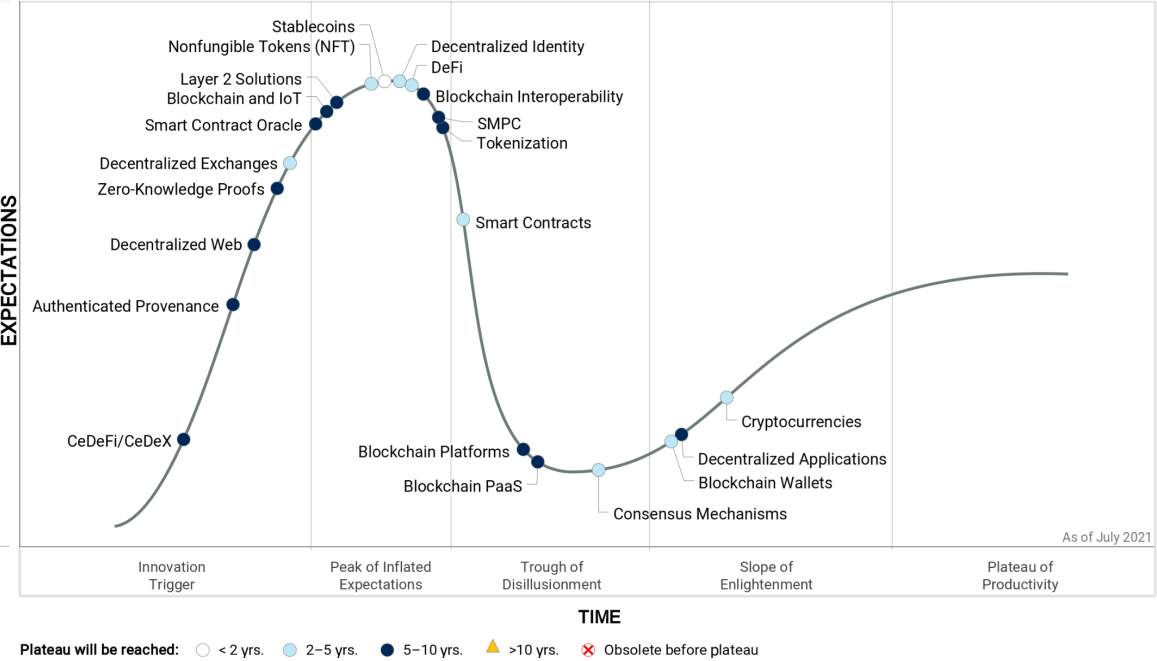
\includegraphics[width=\textwidth]{img/inleiding/gartner-hypecycle.png}
	\caption{\label{fig:gartner}Hype Cycle for Blockchain~\autocite{Gartner2021}}
\end{figure}

In Figuur~\ref{fig:gartner} werd blockchain opgesplitst in 22 verschillende toepassingen. Elke toepassing werd voorgesteld als een punt op de Gartner Hype Cycle: een curve die weergeeft hoe de perceptie rond een hype-technologie evolueert doorheen vijf vaste fases. Elk punt toont aan in welke fase de bijhorende toepassing zich bevindt (x-as) en als gevolg ook hoe hoog de verwachtingen errond zijn (y-as). De kleur van het punt stelt tevens een inschatting voor van hoe snel die toepassing matuur zal worden. 

Merk op dat 9 van de 22 toepassingen zich nog in de eerste opwaartse trend van de curve bevinden.
Die stijging wordt op gang getrokken door  een ``Innovation Trigger'' zoals een proof-of-concept of belangstelling in de media. Men schat het potentieel heel hoog in, hoewel daar op dat moment nog weinig tot niets van in vervulling gebracht is. Hierdoor bereiken de verwachtingen al snel een maximum dat aanzienlijk hoger ligt dan wat de toepassing daadwerkelijk zal kunnen waarmaken: de ``Peak of Inflated Expectations''. Deze schromelijke overschatting zorgt gelukkig wel voor het nodige initiatief om de eerste commerciële projecten op poten te zetten. Een proces dat nog heel riskant is in dit onwtikkelingsstadium.

De ``Trough of Disillusionment'' maakt zijn intrede wanneer de eerste projecten niet het gewenste resultaat opleveren.
De verwachtingen van investeerders gaan de dieperik in door wat voor hen overkomt als mislukte experimenten. Desondanks is het een fase die zich aanbiedt als de geschikte gelegenheid tot onderzoek. Toepassingen, zoals \textit{Smart Contracts} en \textit{Blockchain Platforms (aaS)} komen stilaan \textit{down to earth} komen en vallen daarom mooi binnen de scope van deze paper. Een mix van succesverhalen en mislukkingen zorgen ervoor dat de grootste waanbeelden de deur uit zijn. De eerste commerciële implementaties doen hun intrede op de markt. Ze staan weliswaar nog in hun kinderschoenen, waardoor bovenstaande vraag echt wel als een onderzoeksvraag mag beschouwd worden. 

In de huidige fase is het nog moeilijk om te beslissen of er mee op de trein gesprongen moet worden of niet. Met dit onderzoek kan hopelijk al een voorproefje gevonden worden van wat de ``Slope of Enlightenment''. Op die manier kan blockchain al benut worden voor de voordelen die binnen enkele jaren pas glashelder zullen worden. De ``Plateau of Productivity'' zal dan weer bereikt worden wanneer mainstream implementaties algemeen benut worden.



\section{Onderzoeksdoelstelling}
\label{sec:onderzoeksdoelstelling}

werkstuk

PvA (verslag met aanbevelingen)

vergelijkende studie

in methodologie staat uitgeschreven hoe ik dit resultaat heb nagestreefd

(zie onderzoeksvoorstel)




\section{Opzet van deze bachelorproef}
\label{sec:opzet-bachelorproef}

% Het is gebruikelijk aan het einde van de inleiding een overzicht te
% geven van de opbouw van de rest van de tekst. Deze sectie bevat al een aanzet
% die je kan aanvullen/aanpassen in functie van je eigen tekst.

De rest van deze bachelorproef is als volgt opgebouwd:

In Hoofdstuk~\ref{ch:stand-van-zaken} wordt een overzicht gegeven van de stand van zaken binnen het onderzoeksdomein, op basis van een literatuurstudie.

In Hoofdstuk~\ref{ch:methodologie} wordt de methodologie toegelicht en worden de gebruikte onderzoekstechnieken besproken om een antwoord te kunnen formuleren op de onderzoeksvragen.

% TODO: Vul hier aan voor je eigen hoofstukken, één of twee zinnen per hoofdstuk

In Hoofdstuk~\ref{ch:conclusie}, tenslotte, wordt de conclusie gegeven en een antwoord geformuleerd op de onderzoeksvragen. Daarbij wordt ook een aanzet gegeven voor toekomstig onderzoek binnen dit domein.